%----------------------------------------------------------------------------------------
%	PACKAGES AND OTHER DOCUMENT CONFIGURATIONS
%----------------------------------------------------------------------------------------

\documentclass[12pt]{article}
\usepackage[danish]{babel}
\usepackage{mathtools}
\usepackage[euler]{textgreek}
\usepackage[numbered,final]{mcode}
\usepackage[utf8x]{inputenc}
\usepackage{amsmath}
\usepackage{graphicx}
\usepackage[colorinlistoftodos]{todonotes}
\usepackage[toc,page]{appendix}
%\usepackage{float}
\usepackage{floatrow} % used for adding "Source" to pictures
\usepackage{hyperref} % used for hyperlinks
\usepackage[all]{hypcap}
\usepackage{bm} % used for bold inline matj
\usepackage{lipsum} % used for lorem lipsum
\usepackage[final]{pdfpages} % used for including PDF's
\usepackage{geometry}
\usepackage{listingsutf8}
\usepackage{listings}
\usepackage{blindtext}
\usepackage{enumitem}
\usepackage{color} %red, green, blue, yellow, cyan, magenta, black, white
\definecolor{mygreen}{RGB}{28,172,0} % color values Red, Green, Blue
\definecolor{mylilas}{RGB}{170,55,241}
\hypersetup{colorlinks=true, linkcolor=black}

% Page margins
\geometry{verbose,tmargin=1in,bmargin=1in,lmargin=1in,rmargin=1in,headsep=0.35in}

\begin{document}
	
	\begin{titlepage}
		
		
		
		\newcommand{\HRule}{\rule{\linewidth}{0.5mm}} % Defines a new command for the horizontal lines, change thickness here
		\setlength{\topmargin}{0in}
		\centering % Center everything on the page
		
		%----------------------------------------------------------------------------------------
		%	HEADING SECTIONS
		%----------------------------------------------------------------------------------------
		\textsc{\LARGE Aarhus universitet}\\[1.5cm] % Name of your university/college
		\textsc{\Large Adaptive Control and Automation}\\[0.5cm] % Major heading such as course name
		\textsc{\large 7. Semester}\\[0.5cm] % Minor heading such as course title
		
		%----------------------------------------------------------------------------------------
		%	TITLE SECTION
		%----------------------------------------------------------------------------------------
		
		\HRule \\[0.4cm]
		{ \huge \bfseries ACA projekt}\\ % Title of your document
		\HRule \\[1cm]
		
		%----------------------------------------------------------------------------------------
		%	AUTHOR SECTION
		%----------------------------------------------------------------------------------------
		
		\begin{minipage}{0.4\textwidth}
			\begin{flushleft} \large
				\emph{Gruppemedlemmer:}\\
				Daniel Tøttrup \\
				Stinus Lykke Skovgaard \\
			\end{flushleft}
		\end{minipage}
		~
		\begin{minipage}{0.4\textwidth}
			\begin{flushright} \large
				\emph{AUID} \\
				au544366\\
				au520659\
			\end{flushright}
		\end{minipage}\\[5cm]
		
		%----------------------------------------------------------------------------------------
		%	LOGO SECTION
		%----------------------------------------------------------------------------------------
		
		
\includegraphics[scale=0.5]{Img/logo.jpg}\\[1cm]
		
		%----------------------------------------------------------------------------------------
		%	DATE SECTION
		%----------------------------------------------------------------------------------------
		
		{\large \today}\\[0.5cm] % Date, change the \today to a set date if you want to be precise
		
		
		\vfill % Fill the rest of the page with whitespace
		
	\end{titlepage}
	
\newpage
\tableofcontents
\newpage
\listoffigures
\newpage

\hypersetup{linkcolor=blue}



%!TEX root = ../../Main.tex
\graphicspath{{Chapters/Indledning/}}
%-------------------------------------------------------------------------------

\section{Indledning}
Til dette eksamensprojekt var der opstillet nogle krav til selve systemet, som vi skulle arbejde på. Systemet skulle være et dynamisk system, med mindst én pol. Systemet skulle være stabilt, og tilgå mindst én aktuator og én sensor via EV3 hardware, hvor igennem regulatoren også skulle implementeres.\\
Vores første ide til projektet var at lave en ”adaptiv følgebil”. Tanken var, at vores Lego bil kunne holde en bestemt afstand til et objekt i bevægelse, hvor svingende hastighed, skiftende hældning på underlaget, samt ændring af vægt monteret på vores Lego bil, ikke ville påvirke dens adfærd.
Efter vi havde lavet test med udstyret til rådighed, besluttede vi os for at gå i en anden retning. Vi fik nemlig mere præcise målinger fra encoderen monteret inde i motoren, og ønskede derfor at gå videre den som vores sensor. Det betød dog også, at vores Lego bil ikke længere ville være i stand til at følge et objekt i bevægelse, da den ikke længere havde ”øjne” i form af en afstandssensor. \\
Ideen vi gik videre med, blev derfor en Lego bil der vil være i stand til at køre en specifik afstand, upåvirket af f.eks. vægt monteret på Lego bilen eller underlagets hældning. Derfor endte vores system i sidste ende med at bestå af en motor, med en indlagt encoder som sensor. 

	
\newpage


	%!TEX root = ../../Main.tex
\graphicspath{{Chapters/Krav/}}
%-------------------------------------------------------------------------------


\section{Krav}
I dette afsnit beskrives kravene til CSS og hvilken funktionalitet systemet skal have. Der er stillet nogle enkelte krav fra kursets side, hvor nogle af disse krav skal indgå i projektet:

\begin{itemize}
	\item Use In Circuit debug tools
	
	\item Implement Drivers, dealing with time critical parameters.
	
	\item Implement Boot Loaders for updating microcontroller firmware
	
	\item Use USB to interface a microcontroller
	
	\item Use operating systems for microcontrollers
	
	\item Use microcontroller knowledge in a final mini project
	
\end{itemize}

Flere af disse krav er implementeret i CSS. Der er brugt tidskritiske drivers til color sensoren, display modulet og til implementeringen af I2C mellem de to microcontrollers. 

\begin{figure}[H]
	\centering
	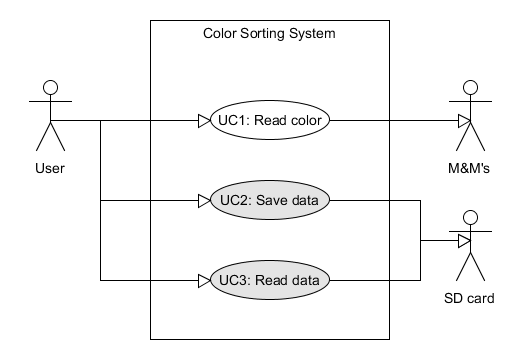
\includegraphics[width = 400pt]{Img/Usecase_diagram.png}
	\caption{Usecase diagram for CSS}
	\label{fig:UsecaseDiagram}
\end{figure}

På \autoref{fig:UsecaseDiagram} ses usecase diagrammet som beskriver sammenhængen mellem aktørerne og de forskellige funktionaliteter der findes for systemet. Uscase 2 og 3 er grå, hvilket betyder at de ikke er implementeret i prototypen. 

\subsection{UC1 - Read Color}
Denne usecase danner ramme for, hvordan CSS måler en farve. Brugeren placerer emne der ønsket aflæst. Brugeren trykker på aflæs-knappen og den aflæste farve kan nu ses talt op på TFT display modulet.

\subsection{UC2 - Save Data}
Denne usecase danner ramme for, at gemme data på SD kort. Brugeren trykker på "Save Data" knappen på skærmen. Data bliver derefter gemt på SD kort.

\subsection{UC3 - Read Data}
Denne usecase danner ramme for, at hente data fra SD kortet. Brugeren trykker på "Load Data" knappen på skærmen. Gemt data bliver hentet fra SD kortet og vist på TFT skærmen.

\subsection{Afgrænsning}
Det skal siges, at usecase 2 og 3 ikke er implementeret i denne protorype. Der er gjort forsøg på at få dem implementeret, men grundet tidspres blev de nedprioriteret. Derudover var det også tænkt fra start, at der ikke skulle være behov for brugerinput for at kunne aflæse farve, men på grund af tidsmangel fik gruppen ikke implementeret et system der kunne fodre CSS med emner. Dette gøres istedet for manuelt og vil i fremtiden skulle noget automatisering af CSS implementeres.


%!TEX root = ../../Main.tex
\graphicspath{{Chapters/Teori/}}
%-------------------------------------------------------------------------------


\section{Color Sensor Module}
Color sensor modulet indeholder både en microcontroller og en color sensor. Til dette projekt har gruppen valgt at bruge en LC Technology TCS3200. Sensoren blev valgt fordi den var på lager i Embedded Stock og den opfylder kravene til sensoren. Den kan opfange de fleste farve, den vil dog i denne prototype kun opfange rød, grøn og blå. Til at styre denne sensor bruges en Arduino mega 2560.

\subsection{LC Technology TCS3200}
LC Technology TCS3200, virker ved at have 8x8 array af fotodioder. 16 fotodioder med et grønt filter, 16 fotodioder med et blåt filter, 16 fotodioder med et rødt filter og 16 fotodioder uden noget filter. De kan alle styres ved at sætte to pins(S2 og S3) høj eller lav. \cite{man:TC3200} Se \autoref{fig:PinSelect}

\begin{figure}[H]
	\centering
	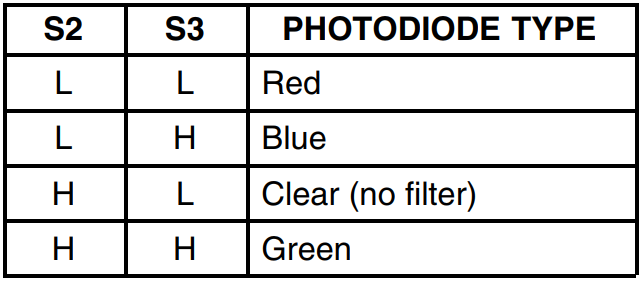
\includegraphics[width = 200pt]{Img/S1S2_color.png}
	\caption{Styring af photodioder}
	\label{fig:PinSelect}
\end{figure}

For at aflæse farveintensiteten, bliver man nødt til at måle på sensorens output pin. Signalet der kommer ud, er et firkantssignal og farveintensiteten er bestemt alt efter, hvor høj frekvensen er. For at se hvilken farve emnet har, bliver man nødt til at aktivere de forskellige fotodioder hver for sig, og tage en måling på output pin'en hver gang man har skiftet fotodiode type. Derefter kan man så sammenligne de tre målinger (Clear bliver ikke målt) og se hvilken er størst. Hvis der skal måles andre farver end rød, grøn og blå, som fx gul, bliver man nødt til at kigge både på grøn og på rød. Hvis begge er lige høje må det være gul. Dog reagerer de forskellige fotodioder forskelligt på hvilken farve man ser på, så der skal der tages højde for. På \autoref{fig:FarveSpektrum} kan man se hvordan de forskellige fotodioder reagerer ved forskellige bølgelændger(farver)\cite{man:TC3200}.

\begin{figure}[H]
	\centering
	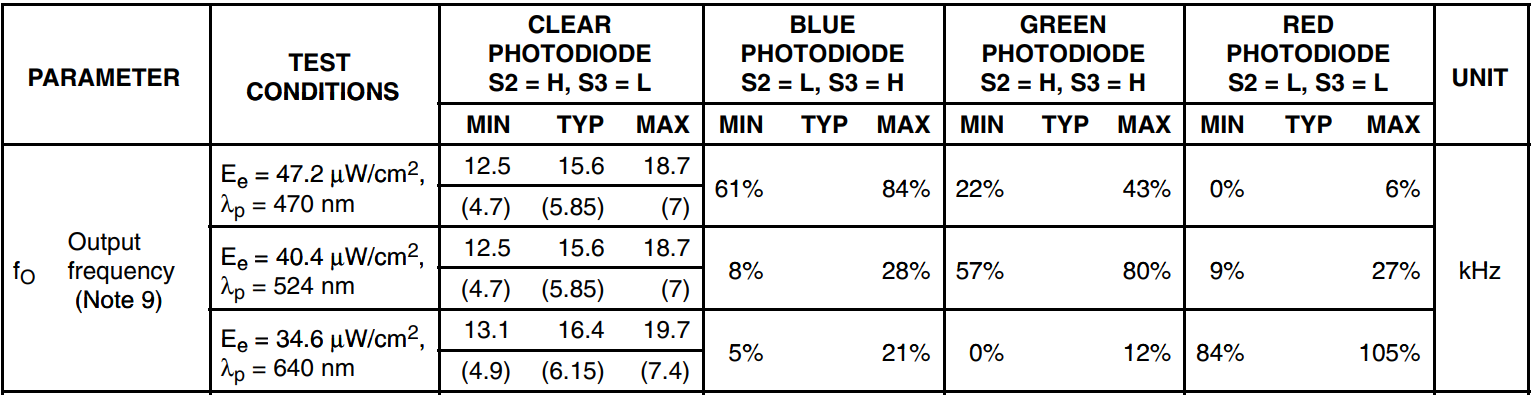
\includegraphics[width = 500pt]{Img/FarveSpektrum.png}
	\caption{Output frekvens ved forskellige farver}
	\label{fig:FarveSpektrum}
\end{figure}

En sidste ting der er værd er at vide om TCS3200, er dens indbygget frequency scaler. Den kan bruges til at styre skaleringen af output signalets frekvens. Skaleringen kan styres ved at sætte S1 og S2 høj eller lav. Til CSS bruges 2\% skalering, da 100\% skalering, ville betyde at output frekvensen kunne komme op over 50kHz. Da databladet skriver at frekvensen typisk ligger under 20KHz ved 100\% frequency scaling er denne høje frekvens underlig, men kunne rettes ved at skifte til 2\% skalering. En lavere frekvens vil være fordelagtig i forhold til at få en præcis måling. \cite{man:TC3200} Se \autoref{fig:Frekvens}

\begin{figure}[H]
	\centering
	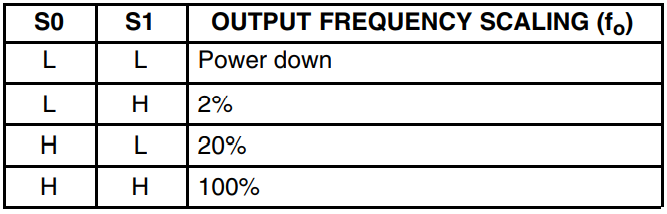
\includegraphics[width = 300pt]{Img/Frekvens.png}
	\caption{Output frekvens skalering}
	\label{fig:Frekvens}
\end{figure}

\subsection{Input Capture}
Input Capture er en metode der ofte bruges i embedded systemer, til at måle på diverse signaler. Til at måle outputsignalet fra TC3200 color sensor bruges denne metode. På \autoref{fig:InputCapture} kan man se en illustartion af hvordan input capture virer.

\begin{figure}[H]
	\centering
	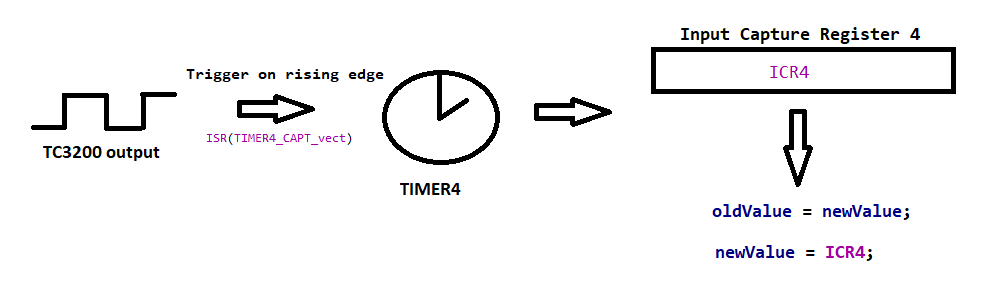
\includegraphics[width = 500pt]{Img/InputCapture.png}
	\caption{Input Capture illustration}
	\label{fig:InputCapture}
\end{figure}

Input Capture \cite{man:mega2560Kap17} fungerer ved at have et interrupt der trigger på rising edge(Dette er tilfældet for CSS). Når dette interrupt bliver kaldt, tages et øjebliksbillede af TIMER4s værdi, som gemmes i Input Capture Register 4. Denne værdi gemmes i en variabel, som bagefter bruges til at beregne en frekvens. 

Derudover skal der også tages højde for overflow, ellers kan man risikerer at en måling ikke vil give en korrekt frekvens. For at udbedre dette problem bruges et anden interrupt, ISR(TIMER4\_OVF\_vect). Det trigger hver gang der kommer overflow, og 65535(16bit max værdi) lægges til newValue. Koden til hvordan frekvensen udregnes kan ses nedenunder.

\newpage
\begin{lstlisting}
ISR(TIMER4_CAPT_vect)
{
	oldValue = newValue;
	newValue = ICR4;
	
	if(newValue < oldValue)
	{
		period = oldValue-newValue;
	}
	else
	{
		newValue + overflow;
		period = oldValue - newValue;
	}
	freq = F_CPU/period;
	FREQFLAG = 1;
}

\end{lstlisting}

Det kan også ses i koden, hvordan overflow værdien lægges til newValue, hvis newValue er mindre end oldValue. FREQFLAG bruges så man altid er sikker på at freq har en ny værdi. FREQFLAG skal selvfølgelig sættes til 0, når man har brugt freq i andre funktioner.

\subsection{Color Sensor Module Software}
For nemt at kunne forstå softwaren brugt til TC3200, er der blevet udarbejdet et data flow diagram, der giver et overblik over dataflowet i softwaren. Dette diagram kan ses på \autoref{fig:DataFlow}. Som det ses i diagrammet, bliver der taget en frekvensmåling for hver farve. Dette gøres, som beskrevet tidligere, ved at sætte S2 og S3 enten høj eller lav. Når en måling er taget, sammenlignes de tre målinger for at se hvilken farve er mest repræsenteret. Derefter sendes en char som enten er 'R', 'G' eller 'B'. Kommunikationen sker via I2C. I2C vil blive uddybt mere i kommunikationsafsnittet. Derefter starter koden forfra igen, og tager en ny frekvensmåling. Source koden kan også ses under bilag\cite{app:ColorSensor}.

\begin{figure}[H]
	\centering
	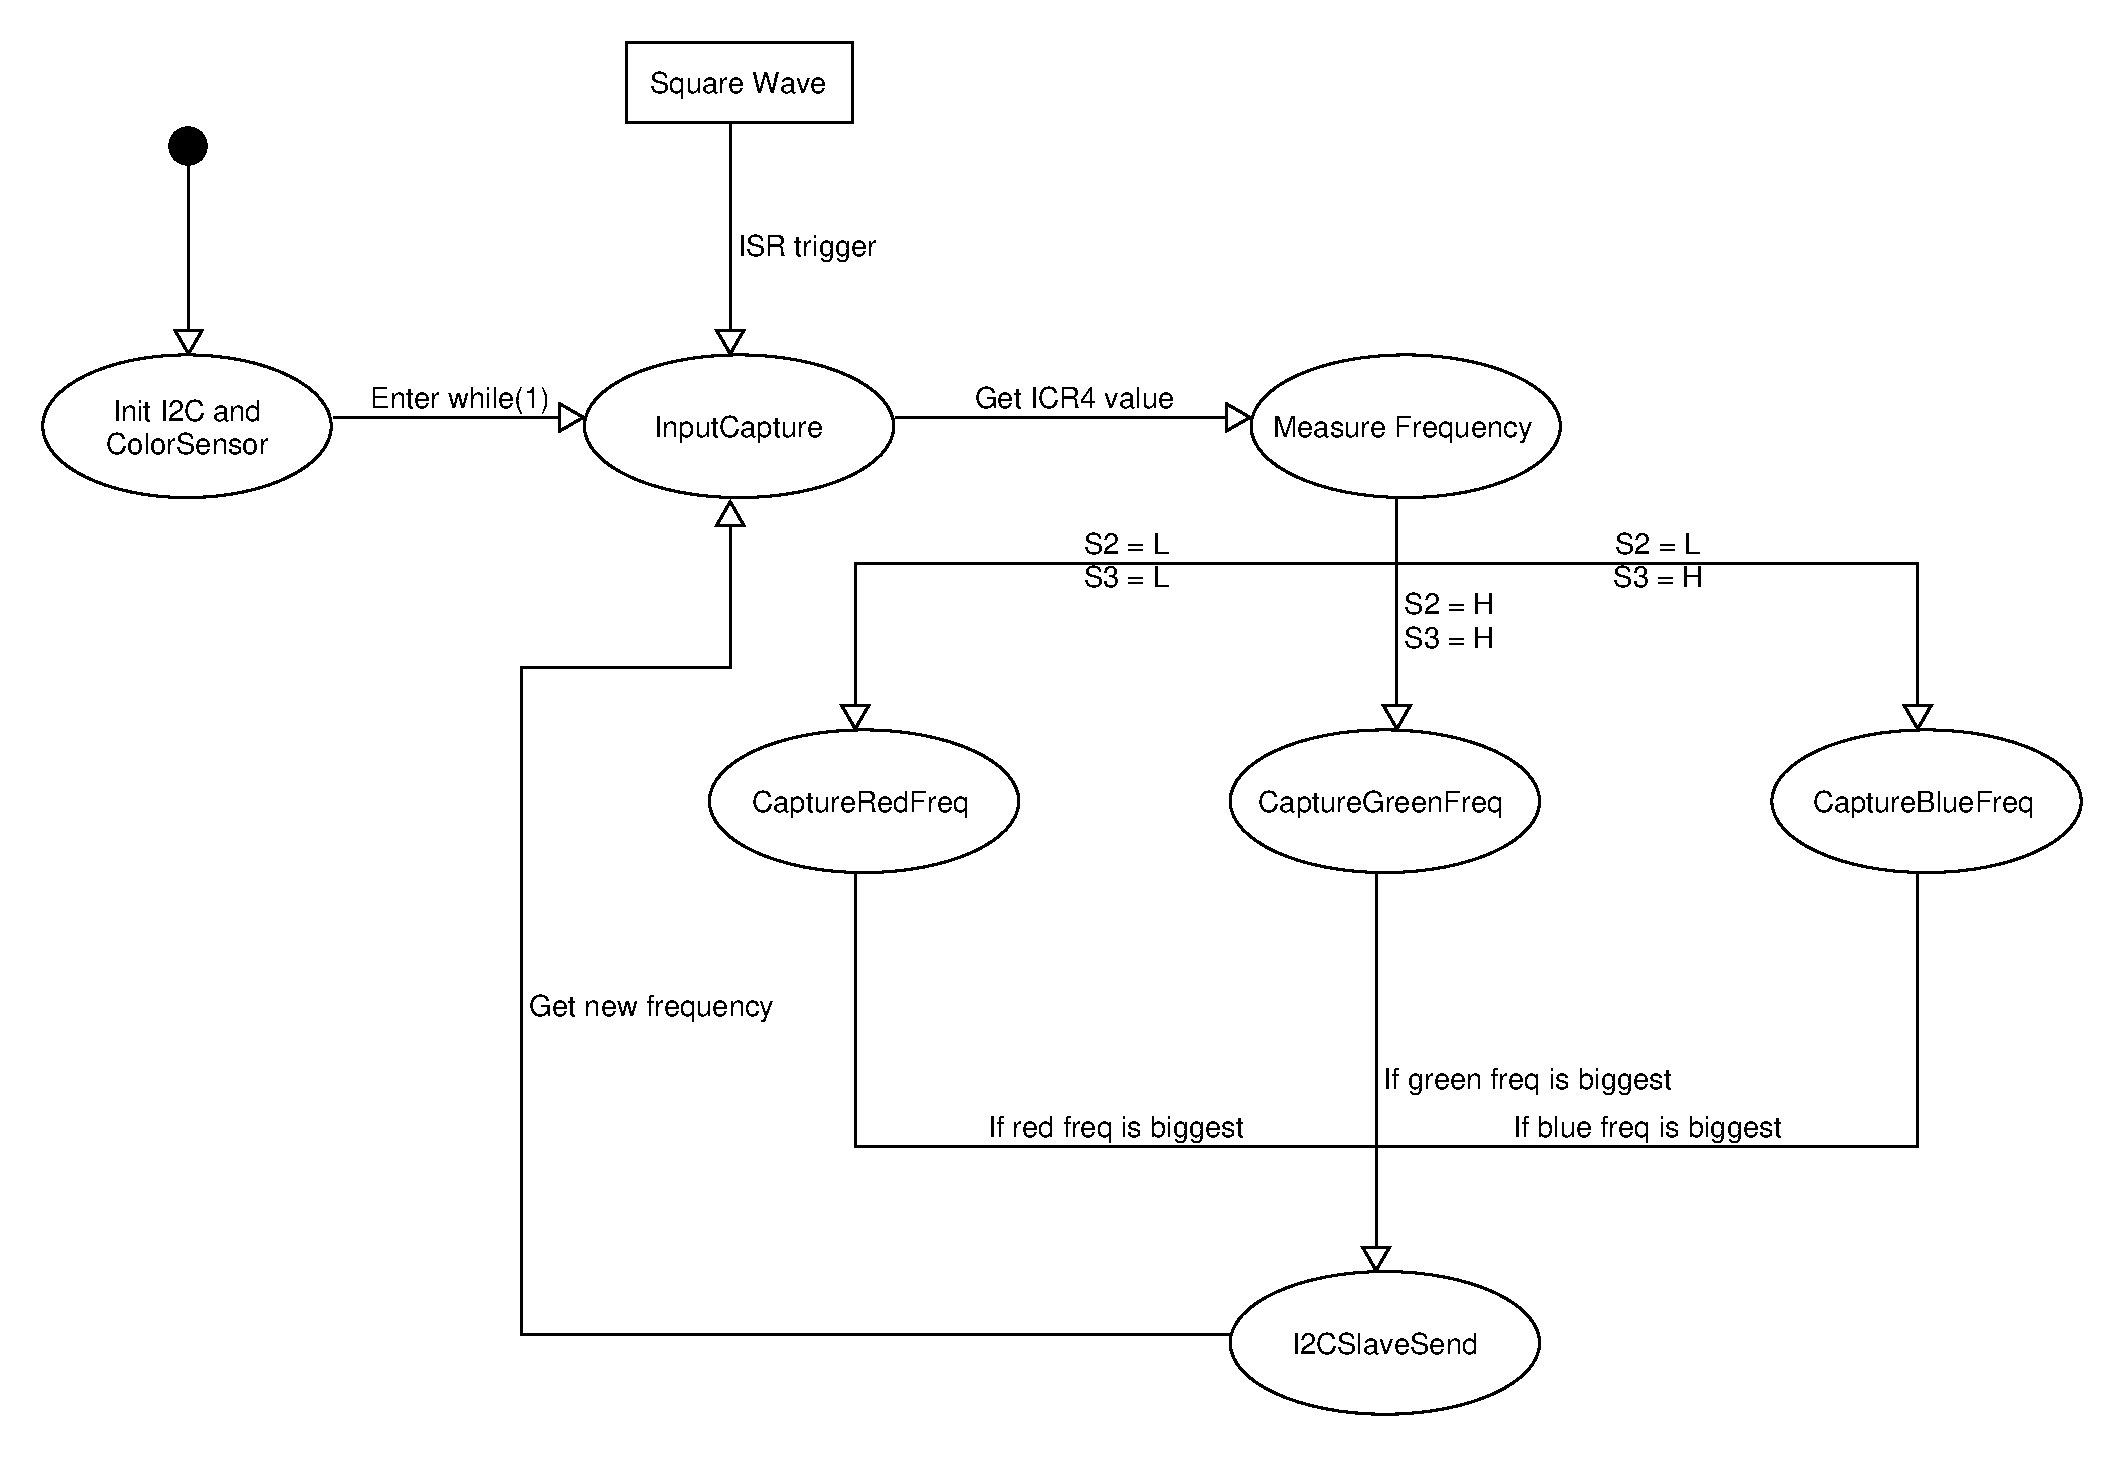
\includegraphics[width = 500pt]{Img/DataFlowDiagram.pdf}
	\caption{Data flow diagram}
	\label{fig:DataFlow}
\end{figure}


\subsection{Test}
En enhedstest er blevet lavet da modulet var færdigt. Resultatet af denne test vil blive fremvist her. Først er input capture softwaren testet ved at bruge en funktions generator til at sende et firkantssignal ind på input capture pin'en. For at se om softwaren kunne aflæse den rigtige frekvens, er der gjort brug af UART kommunikation til en tilsluttet PC. Fra en terminal på PC'en har man kunne aflæse frekvensen fra arduino'en og derfra konstatere at programmet har virket.

\begin{figure}[H]
	\centering
	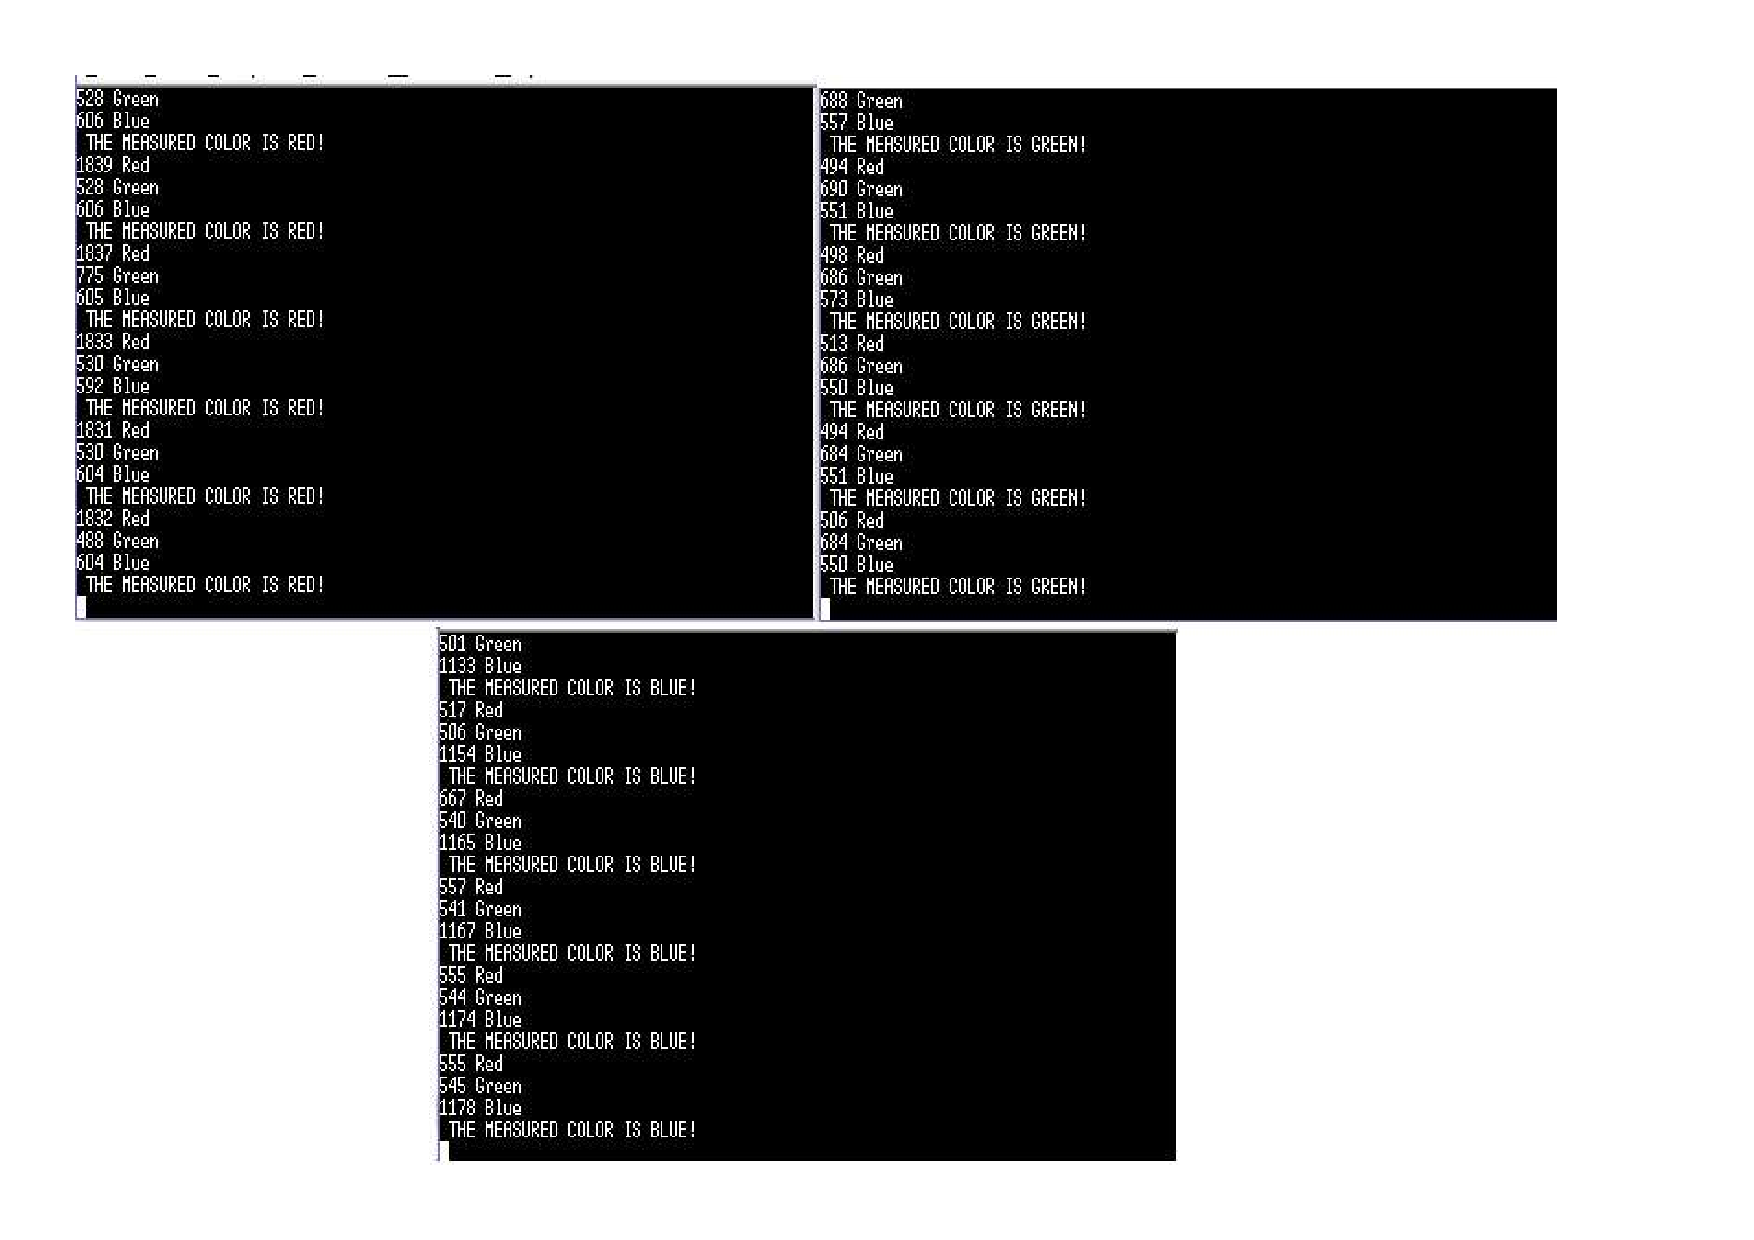
\includegraphics[width = 450pt]{Img/Test_all.pdf}
	\caption{Terminal output ved rød, grøn og blå test}
	\label{fig:Test_all}
\end{figure}

Til test af color sensoren, er der gjort brug af Input Capture programmet sammen med UART kommunikation til en PC. Sensorens output pin blev koblet til input capture pin'en, og tre målinger blev taget, én for hver farve(RGB). Farven med den højeste frekvens blev udskrevet på terminalen, se \autoref{fig:Test_all}. Som farvet forsøgsemne, blev tre forskelligt farvet stykker papir brugt. For at få så godt et resultat som muligt, skulle papiret holdes max 1cm fra sensoren, dog var det grønne papir stadig svært at opfange for sensoren. På \autoref{fig:Test_all} kan man se terminal outputtet fra sensoren. Tallene til venstre for "Red", "Green" og "blue" er frekvensen målt ved den farve. Man kan se hvordan sensoren har svært ved at opfange den grønne farve. Dette skyldes højst sandsynligt at farven ikke var den samme som databladet brugte til at teste med($\lambda = 524 nm$)\cite{man:TC3200}. Udover den grønne farve ikke passede helt, kan sensoren stadig skelne imellem de tre forskllige farver. 

Test opstillingen kan ses på \autoref{fig:Test_opstilling}.

\begin{figure}[H]
	\centering
	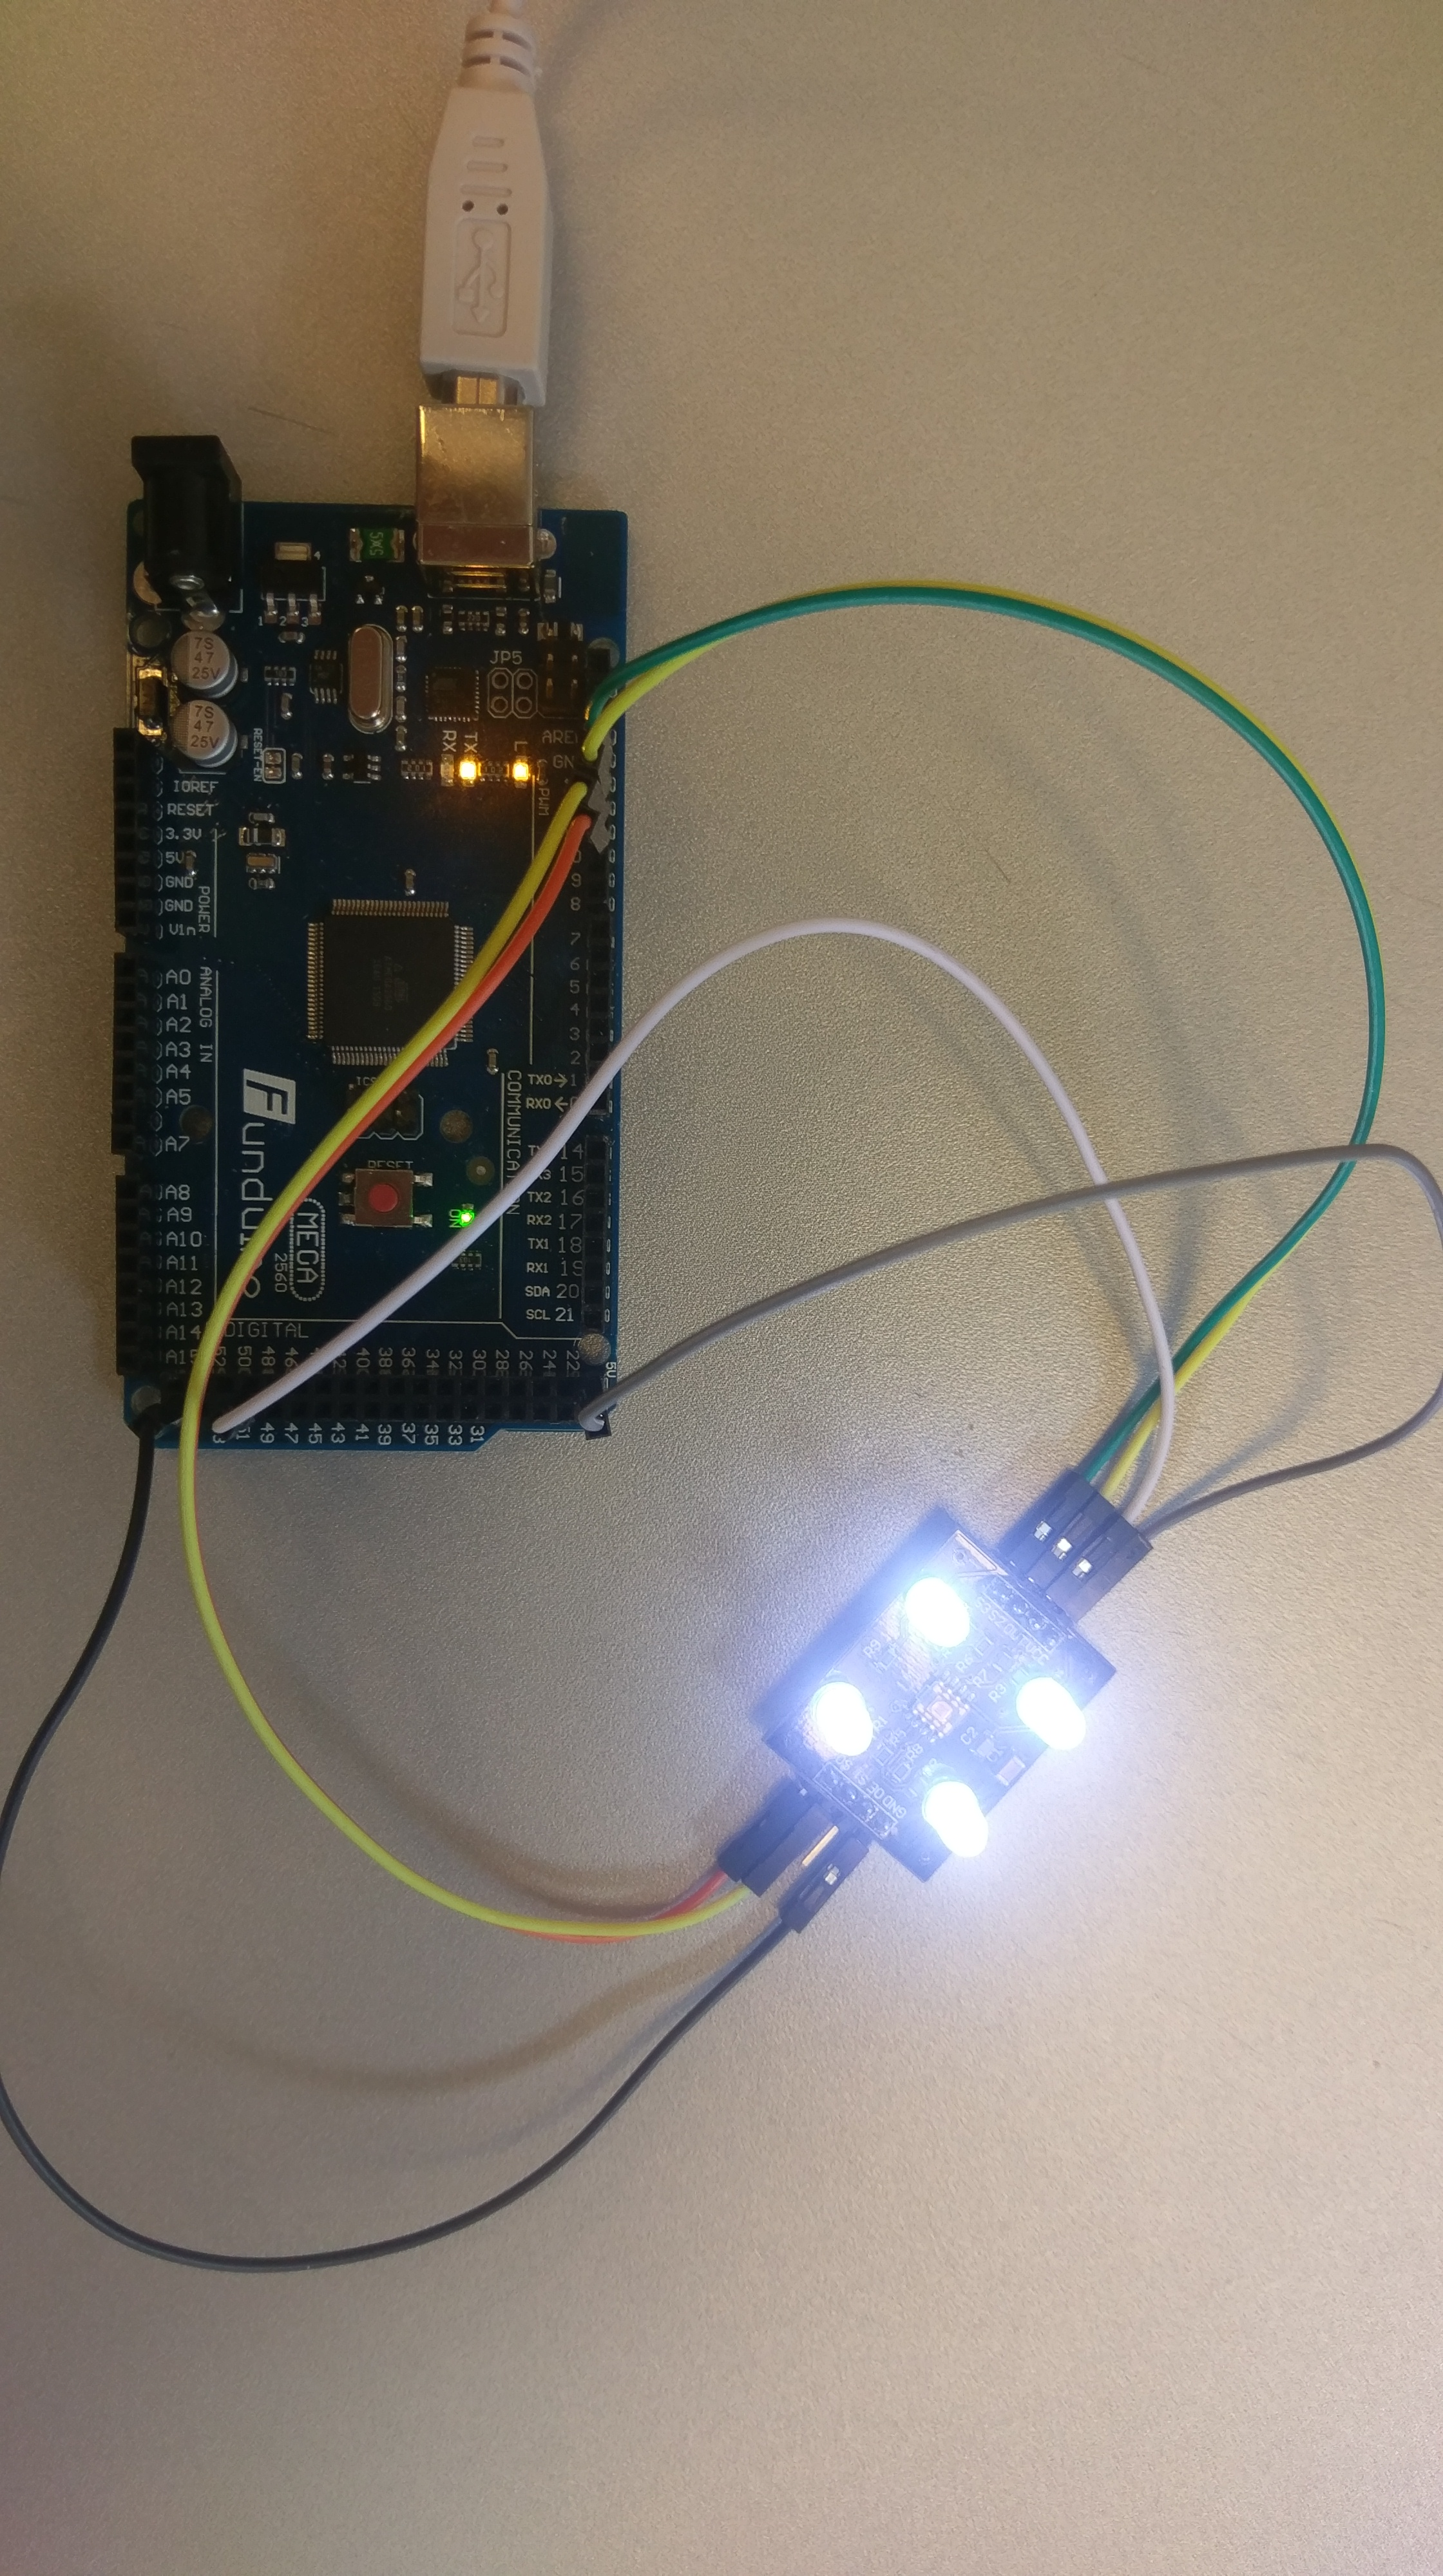
\includegraphics[width = 300pt]{Img/TestOpstilling.jpg}
	\caption{Test opstilling af Color Sensor Modulet}
	\label{fig:Test_opstilling}
\end{figure}



%!TEX root = ../../Main.tex
\graphicspath{{Chapters/Pol-placering/}}
%-------------------------------------------------------------------------------

\section{Pol-placering}
For at designe en lukket sløjfe controller for ens system, har vi gjort brug af pol-placerings princippet. Dette gøres ved at først at bestemme hvilken orden ens system har (første, anden osv.). Ud fra hvilken orden ens system har kan man lave en karakteristik ligning for denne. I vores tilfælde er det et anden-ordens system, hvilket for ligningen til at se således ud:

\begin{equation}
 \frac{wn^2}{s^2+2*\zeta*wn*s+wn^2}
\end{equation}


Derefter skal vi bestemme nogle krav til systemet. Vi har valgt at vores overshoot skal ligge på 5\% og vores settlingtime til 2 sekunder. Disse krav er forskellige fra system til system og bestemmes af hvad systemet skal bruges til. Når vi har valgt vores settlingtime og overshoot kan vi finde polerne for karakteristikligningen. Disse poler skal bruges til at designe vores controller, så den får den rette karakteristik, altså 5\% overshoot og 2 sekunders settlingtime. Nedenunder kan man se blok opbygningen af et system med state-variable feedback.


\begin{figure}[H]
	\centering
	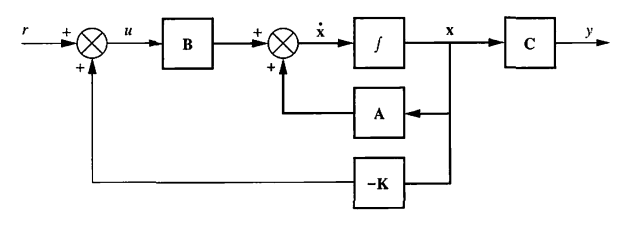
\includegraphics[width = 400pt]{Img/Controller_blok.png}
	\caption{Blok diagram over vores controller}
	\label{fig:Blok_CL}
\end{figure}

Vi gør brug af matlab funktionen place, som kan beregne vores state feedback matrix, K. Dette gør vi ved at indsætte state space variablerne A og B, som vi fandt frem til i starten og polerne fra vores karakteristik ligning. Dermed får vi beregnet vores feedback matrix så den passer med vores krav.
Nu kan vi teste om vores controller fungerer efter hensigten ved at smide et stepinput ind i systemet og kigge på responsen. Dette kan ses på \autoref{fig:StepOfSysSS_cl}.  

\begin{figure}[H]
	\centering
	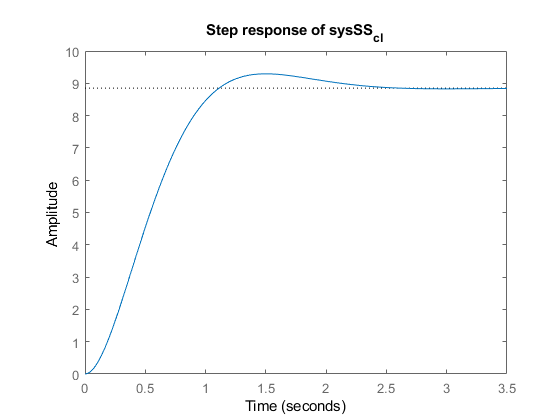
\includegraphics[width = 400pt]{Img/StepOfSysSS_cl.png}
	\caption{Steprespons for closed loop system}
	\label{fig:StepOfSysSS_cl}
\end{figure}



\subsection{Steady state error}

\begin{figure}[H]
	\centering
	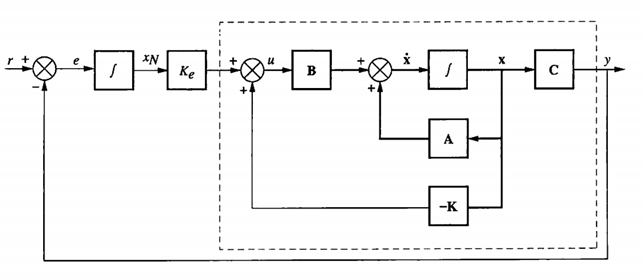
\includegraphics[width = 300pt]{Img/SteadyState_blok.png}
	\caption{Matrix når tredje pol indsættes}
	\label{fig:SteadyStateMatrix}
\end{figure}
For at fjerne steady state error skal en tredje pol indsættes


Man kan se på step responset at der er en stor steady state fejl. Denne fejl kan elimineres ved at indsætte endnu en pol i systemet. Denne pol skal gerne ligge så langt væk fra de eksisterende poler at det ikke har nogen indflydelse på systemets karakteristik. Til vores system vælger vi denne tredje pol til at ligge i -30. 

Da vi tilføjer endnu en pol og dermed også gør det til et tredje ordens system, bliver vi nødt til at lave om på vores state space matricer A, B, C og D. De skal udvides så de kommer til at se ud som på billedet nedenfor.

\begin{figure}[H]
	\centering
	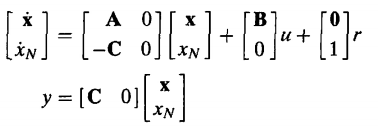
\includegraphics[width = 300pt]{Img/SteadyState_matrix.png}
	\caption{Matrix når tredje pol indsættes}
	\label{fig:SteadyStateMatrix}
\end{figure}

Denne matrix kan også laves på blokform. 

%!TEX root = ../../Main.tex
\graphicspath{{Chapters/Observer/}}
%-------------------------------------------------------------------------------

\section{Observer}
I tidligere afsnit har vi beskrevet hvordan vi har designet vores controller. Men designet af en controller afhænger af at vi har adgang til state variablerne, så vi gennem feedback kan tillægge de ønskede forstærkninger. Måden hvorpå vi fik adgang til vores state variabler i sidste afsnit, vil give os et problem når vi ønsker at implementere vores controller på det virkelige system. På \autoref{fig:cl_system_makeret_plant} kan man se hvordan vi hiver state variablerne ud direkte inde fra systemet, som er omridset med rød. Dette er ikke muligt på et virkeligt system.

\begin{figure}[H]
	\centering
	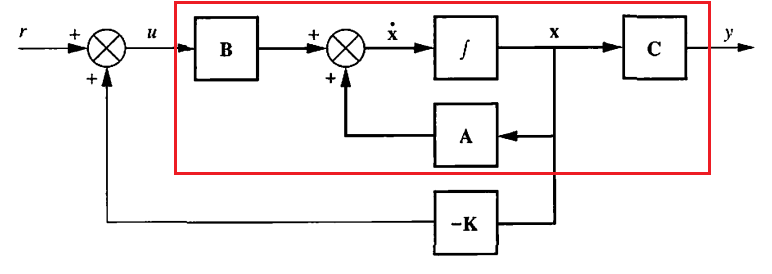
\includegraphics[width = 300pt]{Img/cl_system_makeret_plant.PNG}
	\caption{State space block diagram uden D}
	\label{fig:cl_system_makeret_plant}
\end{figure}


Det er her vores observer design kommer ind i billedet. For hvis ikke det er mulig at tilgå de aktuelle states, grundet f.eks. omkostninger eller opbygningen af systemet. Er det i stedet mulig at estimere de aktuelle states via et observer design. Det er så disse estimerede states, frem for de aktuelle states, der bliver videregivet til controlleren.
På \autoref{eq:Observer_stateSpace_AogB} og \autoref{eq:Observer_stateSpace_C} kan man se observereren som model af systemet. Hvis vi så sammenligner denne model med den faktiske model af systemet, ved at lave en subtraktion \autoref{eq:Subtraktion_A} og \autoref{eq:Subtraktion_C}. Her bliver det tydeligt at forskellen mellem modellerne afhænger af forskellen på den faktiske state og den estimerede state. 
\begin{equation}
\dot{\hat{x}} = A * \hat{x} + B * u
\label{eq:Observer_stateSpace_AogB}
\end{equation}

\begin{equation}
\hat{y} = C * \hat{x}
\label{eq:Observer_stateSpace_C}
\end{equation}

\begin{equation}
\dot{x} - \dot{\hat{x}} = A * (x -\hat{x})
\label{eq:Subtraktion_A}
\end{equation}

\begin{equation}
y -\hat{y} = C * (x - \hat{x})
\label{eq:Subtraktion_C}
\end{equation}

Derfor er det vigtigt at vores estimerede state altid bliver beregnet meget hurtigere end den faktiske state. For at øge hastigheden for konvergensen mellem den faktiske og estimerede state bruger vi et feedback og sammenligner de to outputs se \autoref{fig:Observer_block_diagram} . Fejlen mellem disse to outputs fører vi så tilbage til det afledte af observeres state. På den måde vil systemet forsøge at tvinge denne fejl til 0. Med dette feedback kan vi designe et transient respons som er meget hurtigere det fra det faktiske system. 

\begin{figure}[H]
	\centering
	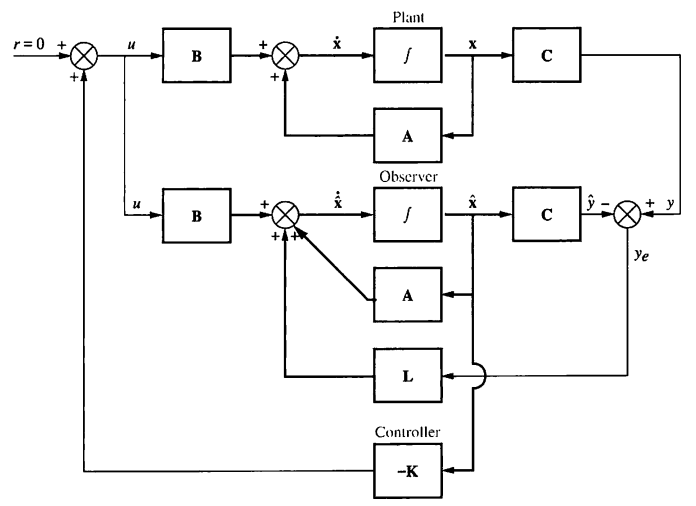
\includegraphics[width = 300pt]{Img/Observer_block_diagram.png}
	\caption{Block diagram af systemet med observer og controller}
	\label{fig:Observer_block_diagram}
\end{figure}

Lige som da vi designede controller vektor, K, består vores observer design også af en konstant vektor, L. Denne vektor, L, skal designes så det transiente respons for observereren er hurtigere end responset fra controlleren. Derfor vælger vi at benytte de samme poler vi placerede for controlleren, vi flytter dem bare tilpas langt ud i det kontinuere domæne, så de bliver hurtige nok til ikke at have en betydelig indflydelse på dynamikken. I vores tilfælde virkerede det at gange polerne med 30. State ligningen for observeren efter L er implementeret kan ses på \autoref{eq:Observer_stateSpace_A_B_L} og \autoref{eq:Observer_stateSpace_C_L} . 
\begin{equation}
\dot{\hat{x}} = A * \hat{x} + B * u + L(y - \hat{y})
\label{eq:Observer_stateSpace_A_B_L}
\end{equation}

\begin{equation}
\hat{y} = C * \hat{x}
\label{eq:Observer_stateSpace_C_L}
\end{equation}

Det kan vi så omskrive til \autoref{eq:Observer_Omskrevet} og \autoref{eq:Observer_Omskrevet_u}

\begin{equation}
\dot{\hat{x}} = (A + B * K - L * C) * \hat{x} + L * y
\label{eq:Observer_Omskrevet}
\end{equation}

\begin{equation}
u =  K * \hat{x}
\label{eq:Observer_Omskrevet_u}
\end{equation}

Det er \autoref{eq:Observer_Omskrevet} og \autoref{eq:Observer_Omskrevet_u} vi implementere i vores system. Denne implementering skete i Simulink og kan ses på \autoref{fig:Discrete_system_med_observer} og \autoref{fig:Discrete_Observer}. Hvor \autoref{fig:Discrete_system_med_observer} er hele systemet med controller, og den lille kasse er lavet som et subsystem. \autoref{fig:Discrete_Observer} er så hvad der sker inde i maven på dette subsystem, som er vores observer.


\begin{figure}[H]
	\centering
	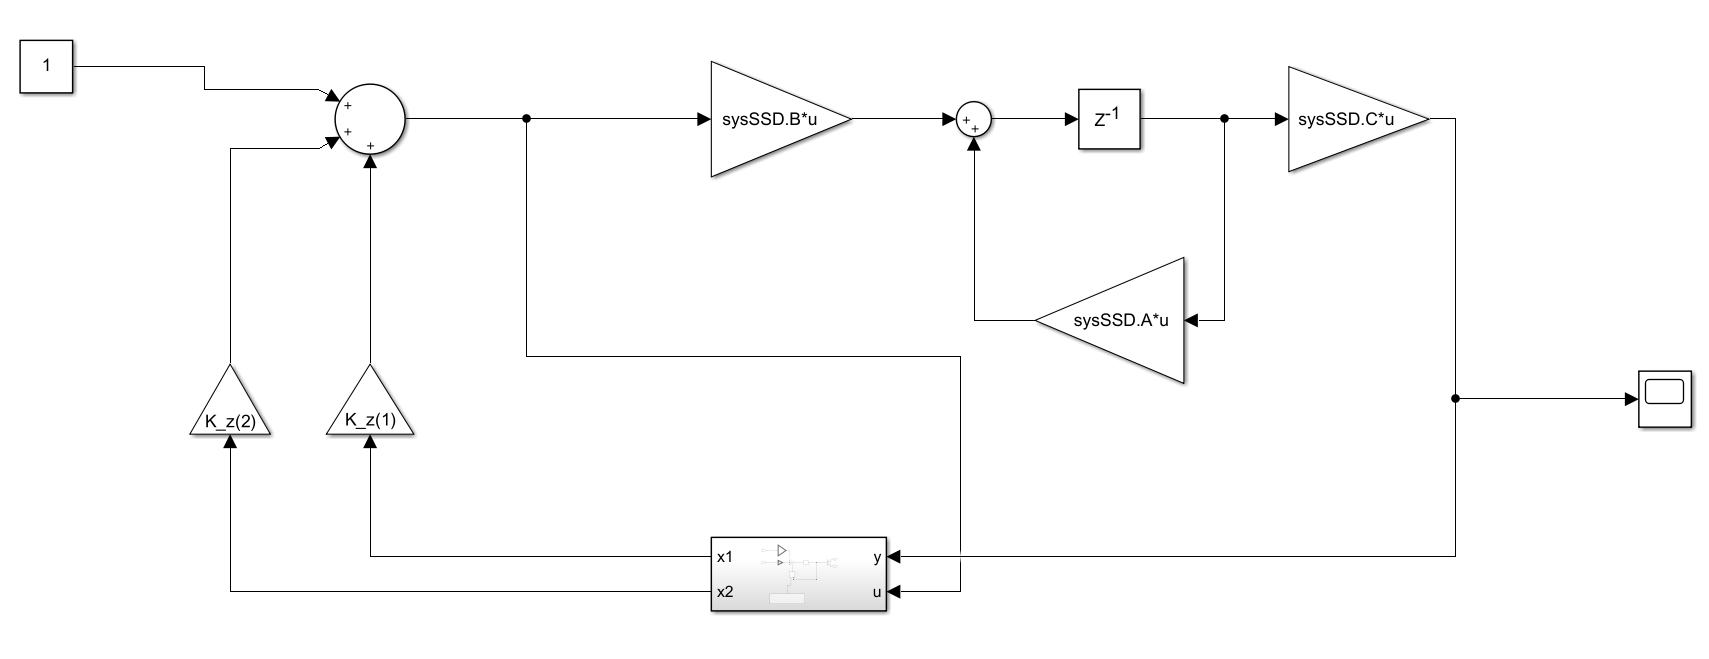
\includegraphics[width = 400pt]{Img/Discrete_system_med_observer.png}
	\caption{Block diagram af systemet med observer og controller}
	\label{fig:Discrete_system_med_observer}
\end{figure}

\begin{figure}[H]
	\centering
	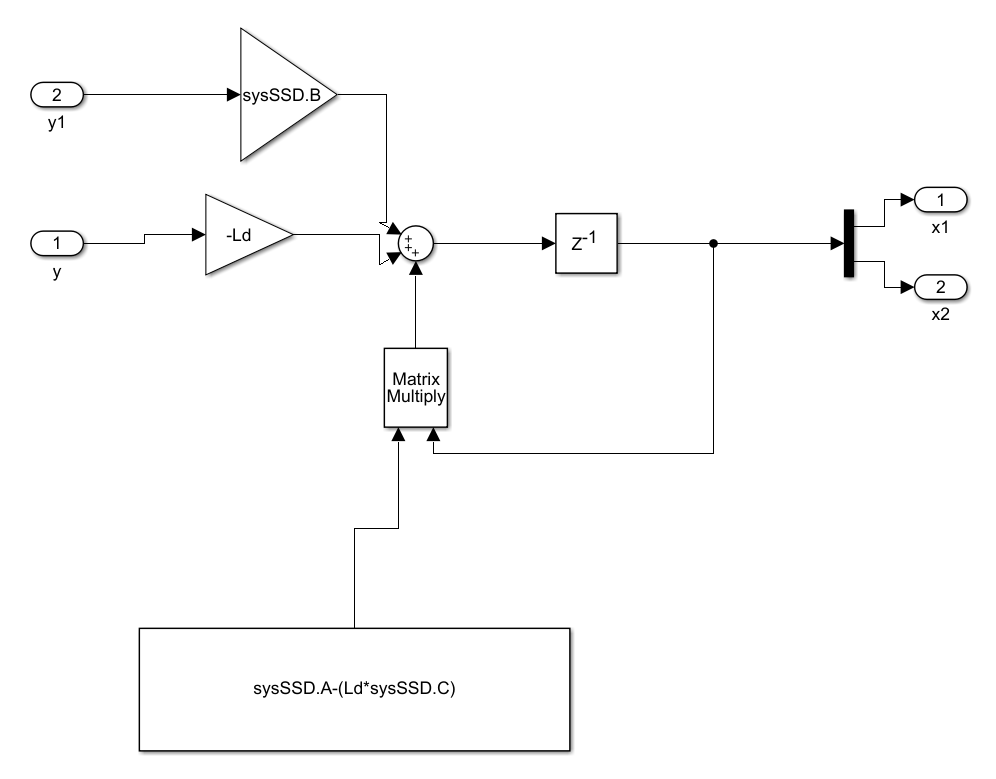
\includegraphics[width = 300pt]{Img/Discrete_Observer.png}
	\caption{Block diagram af systemet med observer og controller}
	\label{fig:Discrete_Observer}
\end{figure}

Da vi ville implementere observer designet på vores system via Simulink, skulle vi først overføre vores system til det diskrete domæne, da vores system kører digitalt. Det gjorde vi ved "c2d" functionen i matlab, som ses i den koden indsat under. Derudover har vi også benyttet os af "pole" functionen som giver polerne ud, samt "place" funktionen som giver en vektor konstant.

\begin{lstlisting}
%% Oberserver design in discrete form
sysSSD=c2d(sysSS,ts,'zoh');%Discrete

ch_eqnD = wn^2/(s^2+2*zeta*wn*s+wn^2); %Charactaristic equation
ch_eqnD = c2d(ch_eqnD,ts,'tustin');
polesD = pole(ch_eqnD);

K_z = place(sysSSD.A,sysSSD.B,polesD);
A_cl = [sysSSD.A-sysSSD.B*K_z];

sysssD_cl = ss(A_cl,sysSSD.B,sysSSD.C,sysSSD.D,ts);

observer_reqZ = polesD/30;

Ld = (place(sysSSD.A',sysSSD.C',observer_reqZ))';
\end{lstlisting}


På \autoref{Discrete_observer_simulering} kan man se simulering af vores observer design i diskret domæne. Det er tydeligt at se at vores system er stabilt, desværre har vi en markant steady state fejl, som vi ikke har kunne fjerne. Hver gang vi har indsat en ekstra pol med forstrækning, blev vores system ustabilt. Dog hvis vi sammenligner med vores closed loop opstilling uden korrigering for steady state fejl får vi meget tæt på det samme resultat. Se \autoref{Continuos_cl_simulering}. Man kan se en lille ændre, hvilket er svært at undgå da, de ektra poler der bliver tilføjet ved observeren påvirker dynamikken en smule.


\begin{figure}[H]
	\centering
	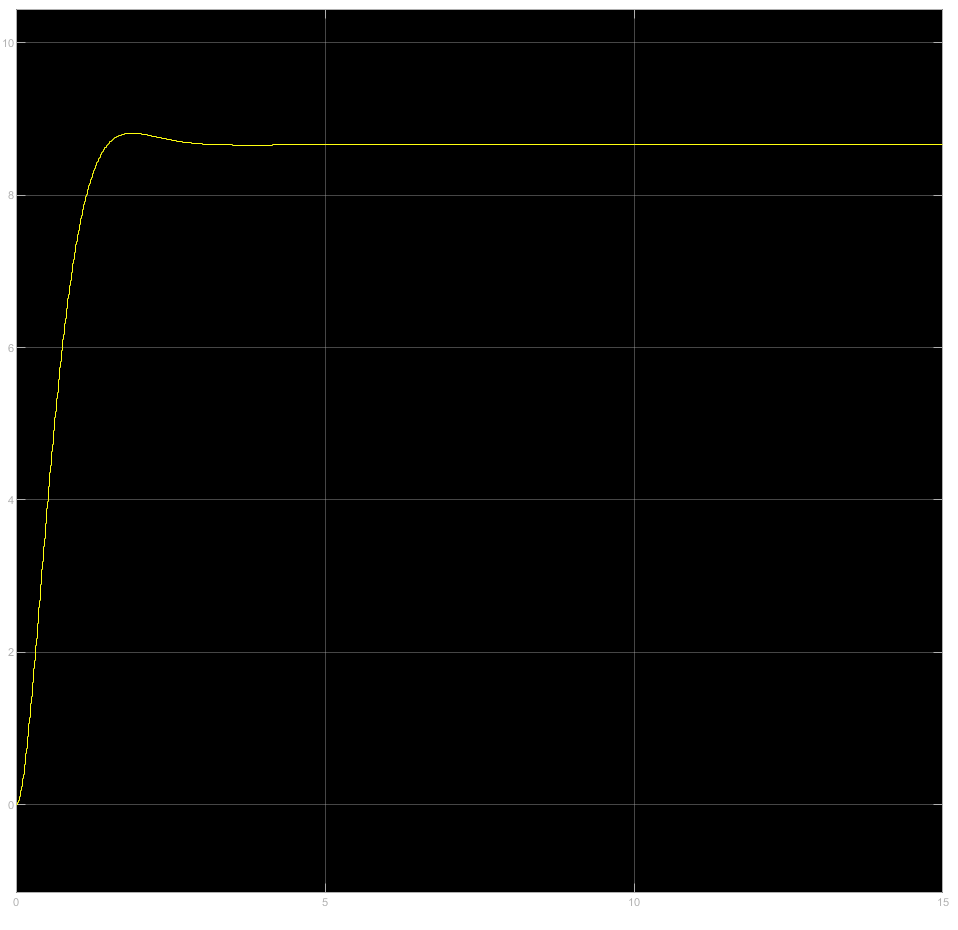
\includegraphics[width = 300pt]{Img/Discrete_observer_simulering.png}
	\caption{Block diagram af systemet med observer og controller}
	\label{Discrete_observer_simulering}
\end{figure}


\begin{figure}[H]
	\centering
	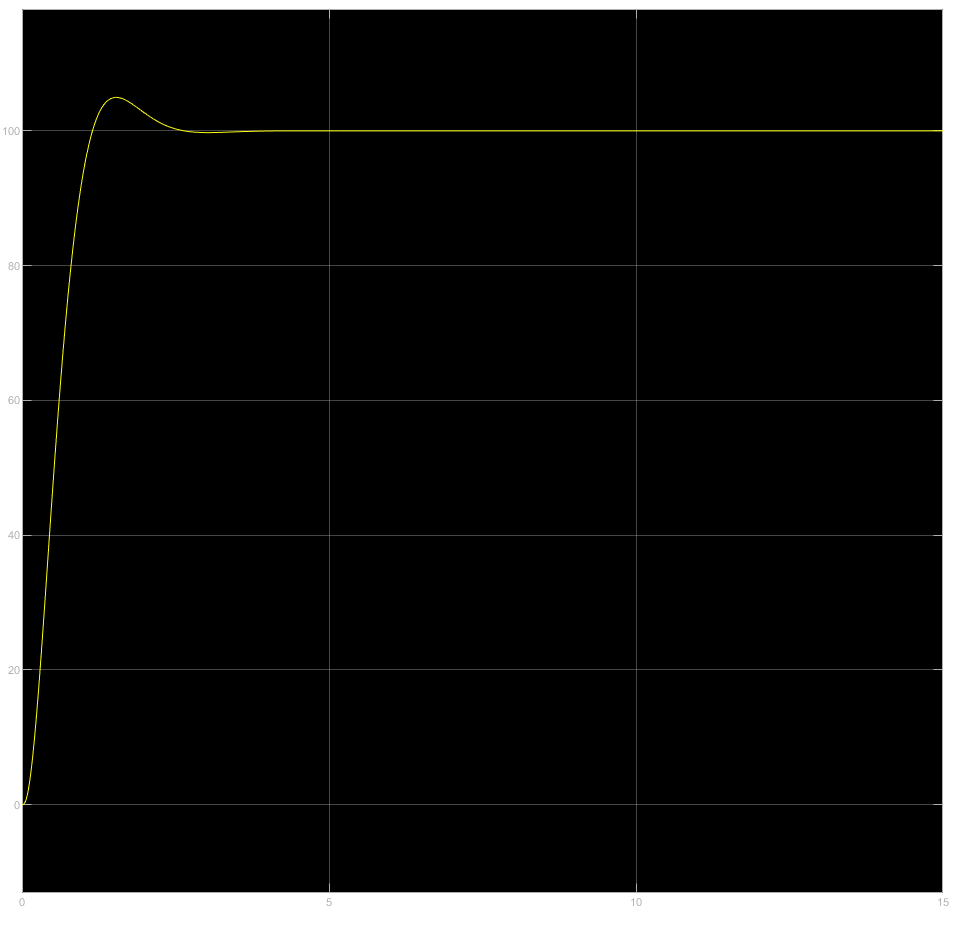
\includegraphics[width = 300pt]{Img/Continuos_cl_simulering.png}
	\caption{Block diagram af systemet med observer og controller}
	\label{Continuos_cl_simulering}
\end{figure}

Til sidst har vi så implementeret dette observer design på vores bil. Simulink opstillingen af dette kan ses på figur \autoref{Discrete_observer_paa_bil}. Bilen opførte sig helt efter forventningnen, og kørte ca 8-9 gange længere end inputet, hvilket passer med steady state fejlen. 

\begin{figure}[H]
	\centering
	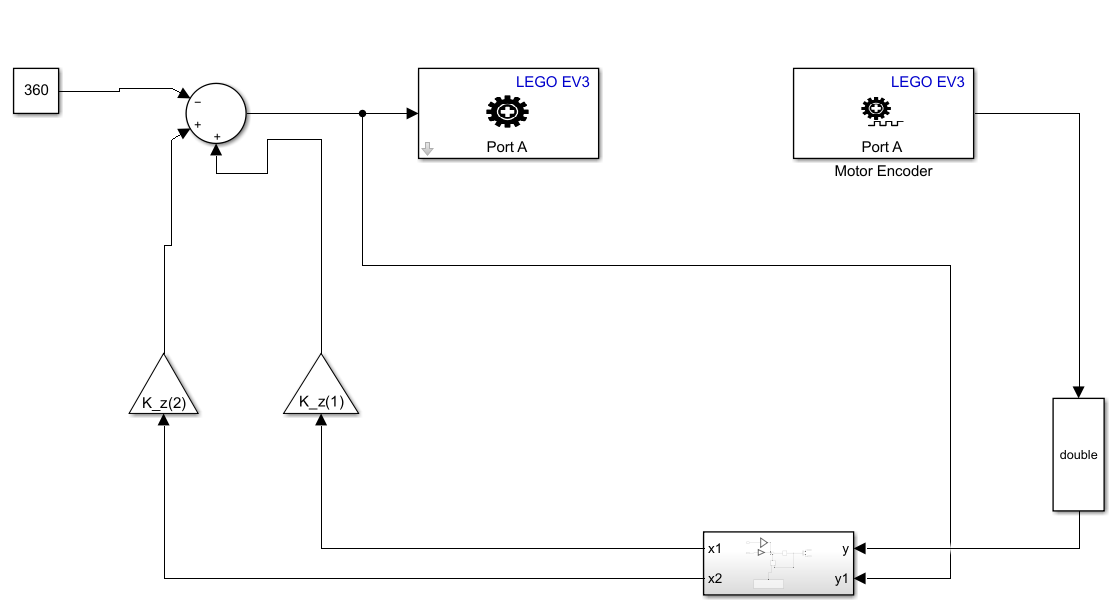
\includegraphics[width = 300pt]{Img/Discrete_observer_paa_bil.png}
	\caption{Block diagram af systemet med observer og controller}
	\label{Discrete_observer_paa_bil}
\end{figure}

%!TEX root = ../../Main.tex
\graphicspath{{Chapters/Overvejelser_for_udvidelser/}}
%-------------------------------------------------------------------------------

\section{Adaptiv controller}
Fra start var det meningen at bilen skulle have en adaptiv controller, så selvom bilen bliver tungere, eller kører på et skævt underlag vil kunne fungerer lige så godt som før. Men på grund af tidsmangel er dette ikke implementeret i bilen, dog er der blevet gjort nogle overvejelser omkring hvordan sådan et system vil se ud. 

\subsection{MIAC}
Vi har i gruppen balgt at bruge det adaptive system MIAC til dette projekt.


\subsubsection{RLS online}
For at bilen skal kunne klare ekstra vægt og et skævt underlag, kan man bruge to forskellige system estimerings algoritmer, RLS online eller RLS offline. For at bilen selv kan regulere for ekstra vægt eller en hældning, vil RLS online give mest mening. RLS online udregner løbende 
 
\begin{figure}[H]
	\centering
	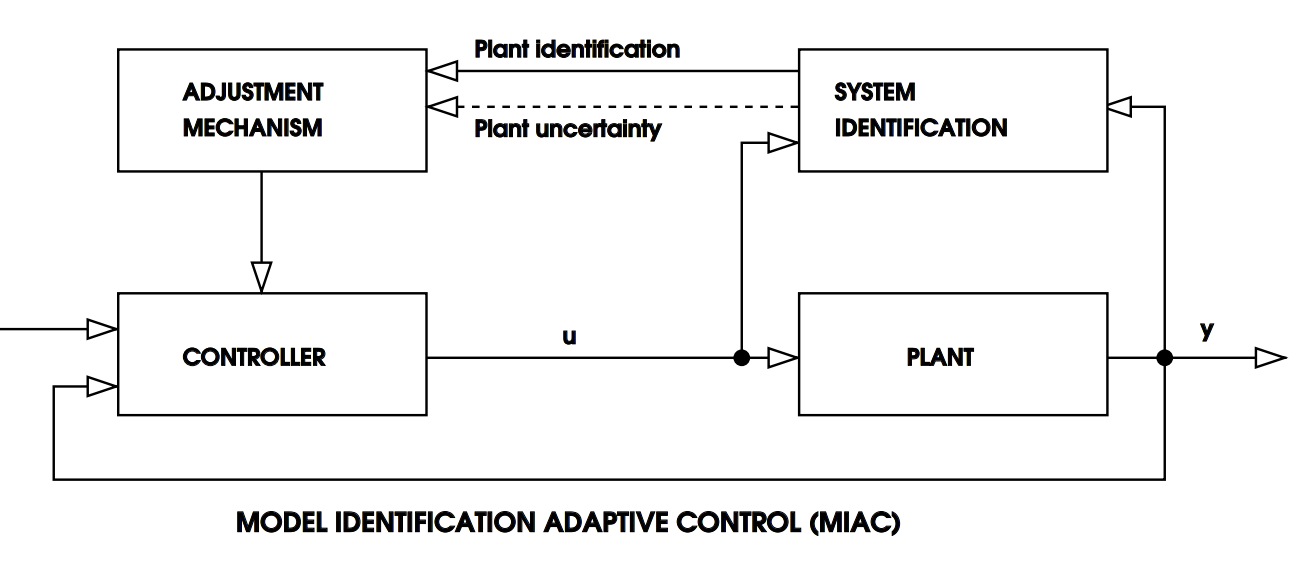
\includegraphics[width = 400pt]{Img/MIAC.png}
	\caption{MIAC blokdiagram}
	\label{fig:MIAC}
\end{figure}

Til system identifikation kan RLS algoritmen bruges. Den fungerer ved løbende at udregne en parameter vektor, som bruges til at opdatere ens controller. Offline RLS vil ikke være det bedste valg til vores bil, da det kræver at man har hele outputtet til at lave estimation på. Det vil sige, at bilen først skal have kørt igennem den rute, man vil have den skal køre.

På \autoref{fig:MIAC} vil RLS algoritmen implementeres i system identifikationsblokken.

\begin{figure}[H]
	\centering
	
\includegraphics[width = 400pt]{Img/ParameterVektor.png}
	\caption{Parameter vektor}
	\label{fig:ParameterVektor}
\end{figure}
 For at udregne parameter vektoren på \autopageref{fig:ParameterVektor}, skal man have sine målte output data og input data, kaldet phi her.
 
 \begin{figure}[H]
 	\centering
 	
\includegraphics[width = 400pt]{Img/InputOutput.png}
 	\caption{Målte output og input værdier}
 	\label{fig:InputOutput}
 \end{figure}
 Men da det kræver meget computerkræft at invetere matricer omskrives ligningen for thetahat.
 
  \begin{figure}[H]
 	\centering
 	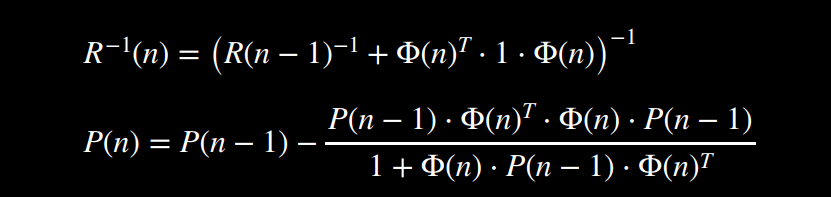
\includegraphics[width = 400pt]{Img/P_rls.png}
 	\caption{Formel for thetahat for RLS online}
 	\label{fig:P_rls}
 \end{figure}
 
 I matlab kan det implementeres på denne måde:
 
 \begin{lstlisting}
 	%Initializering PsiPsi
 	PsiPsi = Psi'*Psi;
 	PsiY = Psi'.*output(1);
 	est_out(1)=0;
 	%Implementation af det digitale filter
 	for n = 2:length(Step)-1
 	
 	Psi_y = [-output(n) Psi_y(1:end-1)];
 	Psi_u = [Step(n-1) Psi_u(1:end-1)];
 	Psi=[Psi_y Psi_u];
 	
 	%Opdater paramter estimation
 	P=P-P*Psi'*Psi*P./(1+Psi*P*Psi');
 	K=P*Psi';
 	Thetahathat=Thetahathat+K*(output(n+1)-Psi*Thetahathat);
 	
 	est_out(n)=Psi*Thetahathat; %Model output y_m(n)
 	end
 \end{lstlisting}
%!TEX root = ../../Main.tex
\graphicspath{{Chapters/Konklussion/}}
%-------------------------------------------------------------------------------

\section{Diskussion}
Igennem projektet har vi stødt på flere forskellige problemer. Et af de meget tidskrævende problemer var identifikation af overføringsfunktionen for vores bil. Vores bil accelerede op til max hastighed utrolig hurtigt, hvilket resulteret i at det transiente område af \autopageref{fig:Motor_deg_graf} blev meget smalt. Det betød at vi kun havde nogle få samples til at bestemme overfæringsfunktionen ud fra. Desuden var der også problemer den første motor, som havde en masse slør der resulterede i at den "hoppede", hvilket teknisk set betød at vi havde en ekstra pol. Vi valgte dog at prøve en anden motor, som viste sig næsten at løse problemt. 
EV3 hardwaren har også voldt os problemer. Det har især været at få forbindelse til EV3 over wifi. Det viste sig at være et problem på en af telefonerne, så det blev løst ved at skifte telefon.
Grundet de mange problemer har vi ikke nået så langt som vi havde forventet, dog er der blevet udarbejdet et godt fungerende kontrolsystem.

\section{Konklussion}

Vi har i dette projekt, fået stillet nogle overordnede krav, til hvad vores regulerings system skulle indeholde. Vi har fra staten ville gribe dette projekt simpelt an, da vi hellere ville stå i en situation, hvor projektet skulle udvides, frem for indskrænkes. Efter forskellige test af sensorer og aktuatorer, endte vores system med at bestå af en motor og en encoder, som skulle være i stand til at køre en specifik afstand, upåvirket af vægt eller andre forstyrrelser.\\
Igennem arbejdet med dette system, kom vi bl.a. omkring identifikation af det faktiske system, placering af poler for at opnå ønsket overshoot og settling time, samt design af observer både i kontinuere og diskret domæne. \\
Selvom vi i gruppen løb ind i en del problemer, bl.a. at oprette forbindelse til HW og fjerne steady state fejlen i det diskrete domæne, fik vi alligevel implementeret en velfungerende observer i det diskrete domæne på vores Lego bil, som fungerede efter hensigten. Grundet tidsmangel og mange problemer undervejs, nåede gruppen aldrig at implementere adaptiv regulering af nogen form på systemet. \\
Alt i alt er gruppen meget tilfreds med projektforløbet, da det har været utrolig lærerigt. Det har givet en helt anden indsigt i arbejdet med regulering, end opgaver i timen her givet. 






\begin{flushleft}
	
\end{flushleft}


\bibliographystyle{plain}
\bibliography{Bibliography}	

 
\end{document}